\section{Design} \label{sec:design}

Analysis of the requirements described in section~\ref{sec:requirements} as well as those in \href{https://moodle.insttech.washington.edu/mod/resource/view.php?id=32929}{Lecture 16b} yielded the hierarchy shown in Figure~\ref{fig:hierarchy}.

\begin{figure}[htbp]
    \centering
    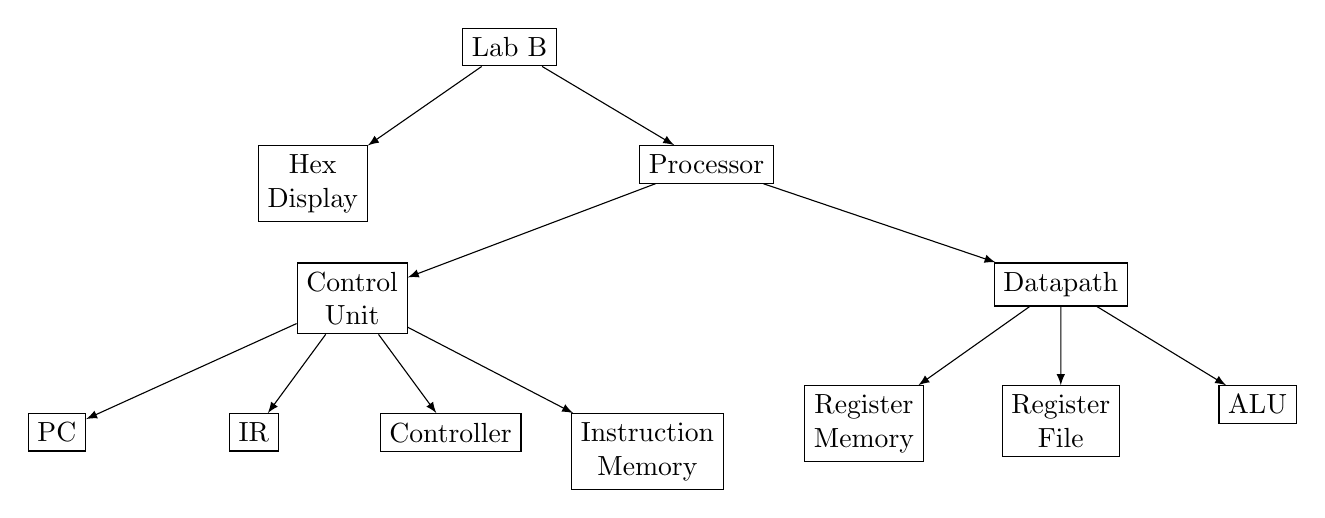
\begin{tikzpicture}[
            every node/.style={rectangle, align=left},
            level/.style={growth parent anchor=south, level distance=1cm},
            level 1/.style={sibling distance=5cm},
            level 2/.style={sibling distance=9cm},
            level 3/.style={sibling distance=2.5cm},
            edge from parent/.style={draw,-latex},
            every child node/.style={anchor=north}]
        \node [draw] (top) {Lab B}
            child {node [draw, align=center] (Hex7Seg) {Hex\\Display}}
            child {node [draw] (Processor) {Processor}
                child {node [draw, align=center] (cunit) {Control\\Unit}
                    child {node [draw] (PC) {PC}}
                    child {node [draw] (IR) {IR}}
                    child {node [draw] (controller) {Controller}}
                    child {node [draw, align=center] (imemlpm) {Instruction\\Memory}}
                }
                child {node [draw] (Datapath) {Datapath}
                    child {node [draw, align=center] (RAM) {Register\\Memory}}
                    child {node [draw, align=center] (RegisterFile) {Register\\File}}
                    child {node [draw] (ALU) {ALU}}
                }
            };
    \end{tikzpicture}
    \label{fig:hierarchy}
    \caption{Top-down Design Methodology}
\end{figure}